\section{The hard pair}
\label{sec:hard-pair}

\subsection{Signed-permutation plants}

Set $q=64$, so $N=q^2$, and write $S_q=\sqrt q\,H_q$ for the unnormalized Sylvester sign matrix. Coordinates in each length-$N$ block are ordered by row-major flattening of a $q\times q$ array, under which $H_N=H_q\otimes H_q$.

A signed permutation is specified by a uniform permutation $\pi$ of $[q]$ and independent uniform signs $\sigma_b$. Associate two sign arrays

\begin{equation}
L_{a,b}=S_q(a,\pi(b))\sigma_b,
\qquad
R_{\pi(b),a}=\sigma_bS_q(b,a).
\label{eq:hard-lr}
\end{equation}

For three independent signed permutations $P_1,P_2,P_3$, define the four positive-plant blocks

\begin{align}
z^{(1)}&=L(P_1),
&z^{(2)}&=R(P_1)\odot L(P_2),
\\
z^{(3)}&=R(P_2)\odot L(P_3),
&z^{(4)}&=R(P_3),
\label{eq:hard-plant}
\end{align}

after flattening. The signed-permutation identities telescope through the three Sylvester transforms and give

\begin{equation}
\Forr(z)=1.
\end{equation}

Replacing $z^{(1)}$ by $-z^{(1)}$ gives an exact negative plant with value $-1$.

Each array entry in Eq.~\eqref{eq:hard-plant} is one binary phase coordinate, with $+1$ representing phase zero and $-1$ representing phase $\pi$. The shared $R(P_j)$ and $L(P_{j+1})$ factors correlate adjacent grids so that their signed-permutation indices contract through the intervening Sylvester transform. Figure~\ref{fig:phase-plant} shows one deterministic realization at the theorem value $q=64$.

\begin{figure*}[t]
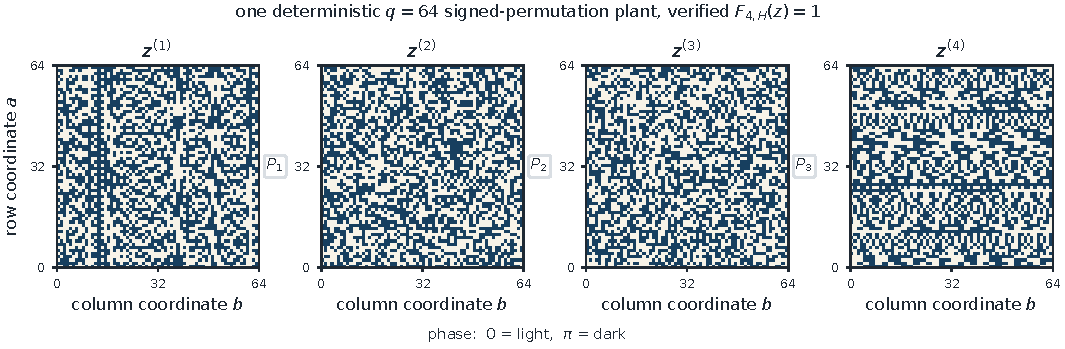
\includegraphics[width=\textwidth]{figures/signed_permutation_phase_grids.pdf}
\caption{One deterministic positive signed-permutation plant at $q=64$. The four panels display the $64\times64$ coordinate arrays $z^{(1)},\ldots,z^{(4)}$, with the two colors denoting phases zero and $\pi$; vector enlargement resolves the individual cells. Adjacent blocks share the indicated signed permutation through their $L(P_j)$ and $R(P_j)$ factors, and an exact integer Walsh--Hadamard contraction verifies $\Forr(z)=1$ for the displayed realization. The square grid represents the logical coordinate pair $(a,b)$ and is not a claim about physical layout.}
\label{fig:phase-plant}
\end{figure*}

\subsection{Attenuation}

Fix the rational attenuation

\begin{equation}
\beta=\frac{19}{25}=0.76.
\end{equation}

Every coordinate in every plant block is multiplied independently by a sign $\eta$ with

\begin{align}
\Pr(\eta=1)&=\frac{1+\beta}{2}=0.88,
\\
\Pr(\eta=-1)&=\frac{1-\beta}{2}=0.12.
\label{eq:hard-attenuation}
\end{align}

The attenuated positive plant has mean forrelation $\beta^4$, while reflection of the first block gives the negative counterpart. Attenuation spreads each exact orbit over many sign strings and reduces the low-degree distinguishability available to a dose-six passive protocol.

\subsection{Conditioning}

Let $\widetilde P_+$ and $\widetilde P_-$ be the two unconditioned attenuated laws. The hard laws used in the theorem are

\begin{align}
P_+&=\widetilde P_+(\,\cdot\mid \Forr\ge1/4),
\\
P_-&=\widetilde P_-(\,\cdot\mid \Forr\le-1/4).
\label{eq:hard-conditioned}
\end{align}

The two laws are therefore supported entirely on the two promise sets. The hard pair is a lower-bound witness and is not part of the definition of the task or the active protocol.

The accepted concentration argument bounds the sum of the two bad-promise probabilities by

\begin{equation}
P_{\mathrm{promise}}
\le 0.002225128406630703.
\label{eq:hard-promise}
\end{equation}

This cost is added once after the unconditioned transcript comparison. Adaptive posterior nodes are not separately conditioned.
